% ----- Consignes exo 1 ----- %
\begin{td-exo}[Inspiré d'un exercice du AIMA] % 1
	Le problème des missionnaires et des cannibales est le suivant:
	3 missionnaires et 3 cannibales sont d'un côté d'une rivière, avec une barque
	qui peut transporter 1 ou 2 personnes à la fois. Trouver une façon de faire
	passer tout ce monde de l'autre côté de la rivière, sans jamais laisser en
	un lieu des missionnaires en minorité par rapport aux cannibales (auquel cas
	il ne resterait plus rien des missionnaires).

	\begin{enumerate}
		\item Formaliser le problème sous la forme de parcours
		d'un problème d'exploration d'un espace d'états:
		\begin{itemize}
			\item Comment représenter un état de problème? Combien d'états
			\og{}potentiels\fg{} votre représentation permet-elle de définir?

			\item Tous les états potentiels sont-ils des états \og{}valides\fg{} du
			problème, c'est-à-dire correspondent à une situation où les missionnaires
			ne sont pas en minorité?

			\item Quel est l'état initial du problème?
			
			\item Quelles actions sont applicables à chaque état (attention une action
			ne doit conduire qu'à un état valide du problème)?

			\item Tous les états valides sont-ils accessibles de l'état initial?

			\item Qu'est-ce qu'un état but?

			\item Quelle pourrait être une fonction de coût pour ce problème?
		\end{itemize}

		\item Dessiner l'espace d'états de ce problème. Finalement, quelle est la taille
		de cet espace d'états? On rappelle que les états d'un problème sont définis
		comme l'ensemble des états atteignables depuis l'état initial.

		\item Donner une solution optimale (i.e.\ de coût minimal) en terme de nombre
		d'actions.

		\item Quel sera le facteur de branchement d'une stratégie de recherche sur
		ce problème?

		\item Une recherche en largeur sur ce problème permet-elle de trouver une solution?
		Si oui, à quelle profondeur et sera-t-elle une solution optimale. Précisez si vos
		réponses dépendent de l'ordre d'exploration des successeurs d'un noeud.

		\item Une recherche en profondeur sur ce problème permet-elle de trouver une solution?
		Si oui, à quelle profondeur et sera-t-elle une solution optimale. Précisez si vos
		réponses dépendent de l'ordre d'exploration des successeurs d'un noeud.
	\end{enumerate}
\end{td-exo}

% ----- Solutions exo 1 ----- %
\iftoggle{showsolutions}{
	\begin{td-sol}[]\ %
		On commence par formaliser nos etats. Voici le tableau représentatif des etats:
		% \begin{center}
		% 	\begin{tabular}{|c|} % chktex 44
		% 		\hline % chktex 44
		% 		Etat
		% 		\hline % chktex 44
		% 		Nombre de cannibales à gauche \(CG\): \(0-3\) \\
		% 		Nombre de missionnaires à gauche \(MG\): \(0-3\) \\
		% 		Position de la barque \(B\): \(\{G, D\}\) \\
		% 		\hline % chktex 44
		% 	\end{tabular}
		% \end{center}
		Le nombre d'etats potentiels est donc de \(4 \times 4 \times 2 = 32\).

		Les contraintes de validité sont les suivantes:
		\begin{itemize}
			\item \(CG \leq MG\) (i.e.\ il y a moins de cannibales que de missionnaires à gauche),
			\item \(CD \leq MD\) (avec \(CD = 3 - CG\) et \(MD = 3 - MG\)).
		\end{itemize}

		L'état initial est \((3, 3, G)\) et l'état but est \((0, 0, D)\).

		Les actions possibles sont:
		\begin{itemize}
			\item traverser avec \(2C\) (si possible),
			\item traverser avec \(1C\) (si possible),
			\item traverser avec \(2M\) (si possible),
			\item traverser avec \(1M\) (si possible),
			\item traverser avec \((1M,1C)\) (si possible).
		\end{itemize}

		Une fonction de coût possible est le nombre de traversées effectuées.

		Le graphe des états est le suivant:\\
		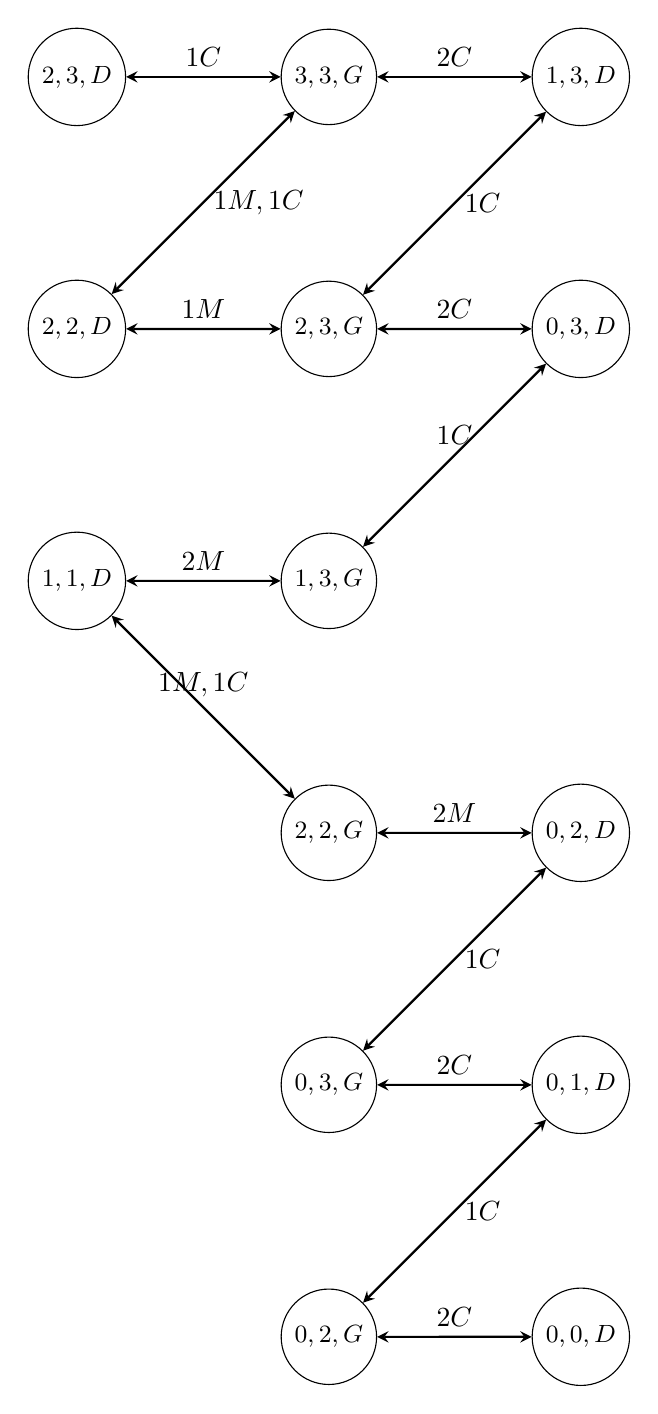
\begin{tikzpicture}[
			state/.style={circle, draw, minimum size=0.5cm, font=\small, align=center},
			edge/.style={<->,>=stealth,thick},
			scale=0.8
		]

		% --- Nodes (placed manually with coordinates) ---
		\node[state] (start) at (0,0) {\(3,3,G\)};
		\node[state] (s1)    at (-4,0) {\(2,3,D\)};
		\node[state] (s2)    at (4,0) {\(1,3,D\)};

		\node[state] (s3)    at (-4,-4) {\(2,2,D\)};
		\node[state] (s4)    at (0, -4) {\(2,3,G\)};
		\node[state] (s5)    at (4, -4) {\(0,3,D\)};

		\node[state] (s6)    at (0,-8) {\(1,3,G\)};
		\node[state] (s7)    at (-4,-8) {\(1,1,D\)};

		\node[state] (s8)    at (0,-12) {\(2,2,G\)};
		\node[state] (s9)    at (4,-12) {\(0,2,D\)};

		\node[state] (s10)   at (0,-16) {\(0,3,G\)};
		\node[state] (s11)   at (4,-16) {\(0,1,D\)};
		
		\node[state] (s12)   at (0,-20) {\(0,2,G\)};
		\node[state] (goal)  at (4,-20) {\(0,0,D\)};

		% --- Edges with labels ---
		\draw[edge] (start) -- node[above]{\(1C\)} (s1);
		\draw[edge] (start) -- node[above]{\(2C\)} (s2);
		\draw[edge] (start) -- node[right]{\(1M,1C\)} (s3);

		\draw[edge] (s4) -- node[right]{\(1C\)} (s2);
		\draw[edge] (s4) -- node[above]{\(1M\)} (s3);
		\draw[edge] (s4) -- node[above]{\(2C\)} (s5);

		\draw[edge] (s5) -- node[above]{\(1C\)} (s6);

		\draw[edge] (s6) -- node[above]{\(2M\)} (s7);

		\draw[edge] (s7) -- node[above]{\(1M,1C\)} (s8);

		\draw[edge] (s8) -- node[above]{\(2M\)} (s9);

		\draw[edge] (s9) -- node[right]{\(1C\)} (s10);

		\draw[edge] (s10) -- node[above]{\(2C\)} (s11);

		\draw[edge] (s11) -- node[right]{\(1C\)} (s12);

		\draw[edge] (s12) -- node[above]{\(2C\)} (goal);

		\end{tikzpicture}
	\end{td-sol}
}{}



% ----- Consignes exo 2 ----- %
\begin{td-exo}[] % 2
	On dispose de 3 cubes \(A, B\) et \(C\) sur une table. Un cube peut être soit
	directement sur la table, soit sur un autre cube. On est dans la situation où
	les cubes \(A\) et \(B\) sont à même la table et le cube \(C\) est posé sur 
	le cube \(A\). On cherche à obtenir la situation où les 3 cubes sont empilés
	de la manière suivante: 
	\begin{itemize}
		\item le cube \(A\) est sur le cube \(C\),
		\item le cube \(C\) est sur le cube \(B\),
		\item le cube \(B\) est sur la table.
	\end{itemize}
	La seule action possible est de déplacer un cube en haut de pile soit sur la 
	table soit sur une autre pile.

	\begin{enumerate}
		\item Formaliser le problème en termes d'états, d'actions, de but et de coût.

		\item Dessiner le graphe des états (représentant l'espace des états).

		\item Quelle est la taille de l'espace des états?

		\item Quel sera le facteur de branchement d'une stratégie de recherche sur
		ce problème?

		\item Que faut-il préciser dans l'algorithme général pour mettre en place 
		une stratégie en largeur? Appliquer l'algorithme de recherche en largeur (pour
		l'ordre des actions issues d'un état (cf.\ liste retournée par XXINSERTCODEHEREXX), % p.actions(n.etat)
		on considèrera en priorité les actions qui créent des empilemments plus hauts
		puis l'ordre alphabétique en cas d'égalité). Préciser l'ordre de génération et 
		d'exploration de chaque noed. Combien de noeuds sont générés et explorés? Combien
		de fois retrouve-t-on l'état initial dans un noeud généré? Dans un noeud exploré?

		\item Mêmes questions pour la recherche en profondeur. Quel problème cela pose-t-il?

		\item On décide maintenant d'ajouter à l'algorithme général de recherche un test 
		évitant de ré-explorer un état déjà exploré. Modifier l'algorithme en conséquence.
		Discuter de l'influence de votre modification sur les stratégies en largeur et en profondeur:
		taille de l'arbre de recherche, de la frontière, ordre d'exploration, complétude de la
		stratégie, optimalité de la solution trouvée.

		% INSERT FOLLOWING CODE HERE
		% Interface Ensemble<Etat> {
		%     Ensemble(); // constructeur d'ensemble vide
		%     contient?(e: Etat): Booleen;
		%     ajouter(e: Etat): void;
		% };

		\item Combien de noeuds sont alors générés et explorés par cet algorithme
		optimisé de recherche en largeur.

		\item Même question pour la recherche en profondeur. 

		\item Proposer une version récursive de l'algorithme (non optimisé) de recherche en profondeur.

		\item Combien de noeuds sont alors générés et explorés par cette version?

		\item On dit que la recherche en profondeur a une complexité spatiale en \(\mathcal{O}(b,d_m)\)
		où \(b\) est le facteur de branchement et \(d_m\) la profondeur maximale à laquelle une 
		solution est cherchée. Si le langage d'implémentation de l'algorithme ne dispose pas d'un
		système de gestion dynamique de la mémoire par \og{}ramasse-miettes\fg{}, quelle
		instruction de suppression faut-il ajouter à l'algorithme récursif pour assurer cette
		complexité spatiale?

		\item On considère à nouveau l'algorithme de recherche en profondeur récursif. Adapter
		cet algorithme pour restaurer la complétude de la recherche sans mémoriser d'états 
		précédemment explorés. On distinguera le cas où l'on peut borner la taille de l'espace
		d'états du cas où l'espace d'états est infini.
	\end{enumerate}

	\(\star\) Pour s'entrainer on pourra reprendre intégralement cet exercice en choisissant comme
	but la situation où le cube \(A\) est sur le cube \(B\), le cube \(C\) étant seul à coté.
\end{td-exo}

% ----- Solutions exo 2 ----- %
\iftoggle{showsolutions}{
	\begin{td-sol}[]\ %
		Notre tableau des etats:
		% \begin{center}
		% 	\begin{tabular}{|c|} % chktex 44
		% 		\hline % chktex 44
		% 		Etat
		% 		\hline % chktex 44
		% 		Position de A: \(\{B, C, T\}\) \\
		% 		Position de B: \(\{A, C, T\}\) \\
		% 		Position de C: \(\{A, B, T\}\) \\
		% 		\hline % chktex 44
		% 	\end{tabular}
		% \end{center}

		L'état initial est \((T, T, A)\) et l'état but est \((C, T, B)\).

		Le nombre d'états est 13, le facteur de branchement est 6.

		Le graphe peut aussi ressembler à:

		\begin{tikzpicture}[
			node distance=2cm and 1.5cm,
			state/.style={
				rectangle, 
				draw=black, 
				thick,
				minimum width=2cm,
				minimum height=1.5cm,
				align=center,
				font=\small
			},
			arrow/.style={->,>=Stealth,thick},
			yellow_num/.style={
				circle,
				fill=yellow,
				inner sep=1pt,
				font=\tiny,
				minimum size=8pt
			},
			red_num/.style={
				circle,
				fill=red!80,
				text=white,
				inner sep=1pt,
				font=\tiny,
				minimum size=8pt
			},
			goal/.style={
				rectangle,
				draw=green!60!black,
				thick,
				fill=green!10,
				minimum width=2cm,
				minimum height=1.5cm,
				align=center,
				font=\small
			}
		]

		% Level 0 (Initial state)
		\node[state] (s1) at (0,0) {\shortstack{CA,B \\ - \\ 0}};
		\node[yellow_num] at (-0.8,0.6) {1};
		\node[red_num] at (-0.8,-0.6) {1};

		% Level 1
		\node[state] (s2) at (-3,-3) {\shortstack{BCA \\ B to C \\ 1}};
		\node[yellow_num] at (-3.8,-2.4) {2};
		\node[red_num] at (-3.8,-3.6) {2};

		\node[state] (s3) at (0,-3) {\shortstack{CB,A \\ C to B \\ 1}};
		\node[yellow_num] at (-0.8,-2.4) {3};
		\node[red_num] at (-0.8,-3.6) {3};

		\node[state] (s4) at (3,-3) {\shortstack{A,B,C \\ C to - \\ 1}};
		\node[yellow_num] at (2.2,-2.4) {4};
		\node[red_num] at (2.2,-3.6) {4};

		% Level 2 from s2
		\node[state] (s5) at (-3,-6) {\shortstack{CA,B \\ B to - \\ 2}};
		\node[yellow_num] at (-3.8,-5.4) {5};
		\node[red_num] at (-3.8,-6.6) {5};

		% Level 2 from s3
		\node[goal] (s6) at (-1.5,-6) {\shortstack{ACB \\ A to C \\ 2}};
		\node[yellow_num] at (-2.3,-5.4) {6};
		\node[red_num] at (-2.3,-6.6) {6};

		\node[state] (s7) at (0,-6) {\shortstack{CA,B \\ C to A \\ 2}};
		\node[yellow_num] at (-0.8,-5.4) {7};

		\node[state] (s8) at (1.5,-6) {\shortstack{A,B,C \\ C to - \\ 2}};
		\node[yellow_num] at (0.7,-5.4) {8};

		% Level 2 from s4 (states 9-14)
		\node[state] (s9) at (1.5,-6) {\shortstack{AB,C \\ - \\ 2}};
		\node[yellow_num] at (0.7,-5.4) {9};

		\node[state] (s10) at (2.5,-6) {\shortstack{AC,B \\ - \\ 2}};
		\node[yellow_num] at (1.7,-5.4) {10};

		\node[state] (s11) at (3.5,-6) {\shortstack{BA,C \\ - \\ 2}};
		\node[yellow_num] at (2.7,-5.4) {11};

		\node[state] (s12) at (4.5,-6) {\shortstack{BC,A \\ - \\ 2}};
		\node[yellow_num] at (3.7,-5.4) {12};

		\node[state] (s13) at (5.5,-6) {\shortstack{CA,B \\ - \\ 2}};
		\node[yellow_num] at (4.7,-5.4) {13};

		\node[state] (s14) at (6.5,-6) {\shortstack{CB,A \\ - \\ 2}};
		\node[yellow_num] at (5.7,-5.4) {14};

		% Level 3 (only shown as we found goal at level 2)
		\node[state] (s15) at (-3,-9) {\shortstack{BCA \\ - \\ 3}};
		\node[yellow_num] at (-3.8,-8.4) {15};

		\node[state] (s16) at (-1,-9) {\shortstack{CB,A \\ - \\ 3}};
		\node[yellow_num] at (-1.8,-8.4) {16};

		\node[state] (s17) at (1,-9) {\shortstack{A,B,C \\ - \\ 3}};
		\node[yellow_num] at (0.2,-8.4) {17};

		% Arrows
		\draw[arrow] (s1) -- (s2);
		\draw[arrow] (s1) -- (s3);
		\draw[arrow] (s1) -- (s4);

		\draw[arrow] (s2) -- (s5);
		\draw[arrow] (s3) -- (s6);
		\draw[arrow] (s3) -- (s7);
		\draw[arrow] (s3) -- (s8);

		\draw[arrow] (s4) -- (s9);
		\draw[arrow] (s4) -- (s10);
		\draw[arrow] (s4) -- (s11);
		\draw[arrow] (s4) -- (s12);
		\draw[arrow] (s4) -- (s13);
		\draw[arrow] (s4) -- (s14);

		\draw[arrow] (s5) -- (s15);
		\draw[arrow] (s7) -- (s16);
		\draw[arrow] (s8) -- (s17);

		% Add legend
		\node[yellow_num] at (8,1) {G};
		\node at (8.8,1) {Generation order};
		\node[red_num] at (8,0.5) {E};
		\node at (8.8,0.5) {Exploration order};

		% Add goal indicator
		\node[color=green!60!black, font=\small\bfseries] at (-1.5,-7.5) {GOAL FOUND};

		\end{tikzpicture}
		On marquera en jaune les étants de génération et en rouge ceux d'exploration.

		On a une fonction qui explore un problème en 
		profondeur et rend un noeux. Voici son implementation:
		\begin{equation*}
			\begin{aligned}
				&\text{Fonction ExplorerProfondeur} (p: \text{Problème}): \text{Noeud} \\
				&\text{racine} \leftarrow \text{NouveauNoeud} (p.\text{etatInitial}, null, null, 0) \\
				&\text{retourner ExplorerRec(racine)}; % chktex 36
				\\ \\
				&\text{Fonction ExplorerRec} (n: \text{Noeud}): \text{Noeud} \\
				&\text{si } p.\text{but}?(n.\text{etat}) \text{ alors }\\
				&\qquad \text{retourner } n; \\
				&\text{sinon} \\
				&\qquad \text{pour chaque } a \text{ dans } p.\text{actions}(n.\text{etat}) \text{ faire} \\
				&\qquad\qquad \text{res} \leftarrow \text{ExplorerRec}(\text{NouveauNoeud}(a.\text{resultat}(n.\text{etat}), n, a, n.\text{cout} + a.\text{cout})); \\
				&\qquad\qquad \text{si res} \neq \text{null alors retourner res}; \\
				&\qquad \text{fin pour} \\
				&\qquad \text{retourner null}; \\
			\end{aligned}
		\end{equation*}
		Une fois de plus, pour éviter de ré-explorer des états, on suppose disposer 
		d'une fonction qui teste l'appartenance d'un état à ses parents.

		On modifie donc l'algorithme précédent en rajoutant la ligne suivante
		au début de la boucle:
		\begin{equation*}
			e' \leftarrow a.\text{resultat}(n.\text{etat}); \\
			\text{si non } (n.\text{AppartientEtatAncetres}(e',n)) \text{ alors } \\
			\qquad \text{ajouter } (e',n) \text{ à la liste des états explorés};
		\end{equation*}
		On aurait aussi pu la rajouter avant l'appel récursif
		avec la modification suivante:
		\begin{equation*}
			\text{si AppartientEtatAncetres}(n.\text{etat}, n.\text{parent}) \text{ alors retourner }null;
		\end{equation*}

		Supposons maintenant qu'on utilise cette version optimisée (la première),
		alors on trouve la solution après seulement 4 noeuds générés et explorés. % 12

		% pour le 13, c l'algo 1 encore mais avec un free apres les return null

		% pour le cas avec une profondeur max, ie pour la completude,
		% on ajoute un parametre \(b\) à la fonction recursive
		% et on ajoute la condition suivante au début de la fonction:
		% si b = 0 alors retourner null;
		% et on rajoute b - 1 dans l'appel recursif

		% ensuite on appelle recursivement avec une profondeur max
		% qui augmente jusqu'à trouver une solution

	\end{td-sol}
}{}

% ----- Consignes exo 3 ----- %
\begin{td-exo}[Taquin] % 3
	Modéliser le jeu du Taquin comme un problème d'exploration d'espace d'états.
\end{td-exo}

% ----- Solutions exo 3 ----- %
\iftoggle{showsolutions}{
	\begin{td-sol}[]\ %
		% PLACEHOLDER
	\end{td-sol}
}{}